\documentclass[a4j,titlepage]{jarticle}
\usepackage[dvipdfmx]{graphicx}
\usepackage{ascmac}
\usepackage{float}
\usepackage{amssymb}%にやりイコールを使う
\usepackage{multirow}
\usepackage{multicol}
%\usepackage{color}

\begin{document}

\title{2022 年度 3 回生前期学生実験 HW  \\ \bf team02 方式設計仕様書}
% ↓ここに自分の氏名を記入
\author{方式設計仕様書作成者:植田健斗\\
グループメンバー:\\伊藤舜一郎 (学籍番号:1029-32-7548)
\\植田健斗 (学籍番号:1029-32-6498)}
\西暦
\date{提出期限:5月12日18時 提出日: \today} % コンパイル時の日付が自動で挿入される
\maketitle
\newpage

\section{概要}
授業資料の仕様を満たすプロセッサを作った。このプロセッサをもとにして、今後拡張機能の追加を目標とする。
授業資料の仕様に加えて、以下の処理を実現するプロセッサの作成を目標とする。
\begin{itemize}
\item 5段のパイプライン処理の設計をする。
\item 即値命令ADDIを実装する。
\end{itemize}

\section{命令セット・アーキテクチャ}
命令セットアーキテクチャは以下の図\ref{instructionSet}のようになる。

\begin{figure}[H]
    \begin{center}
    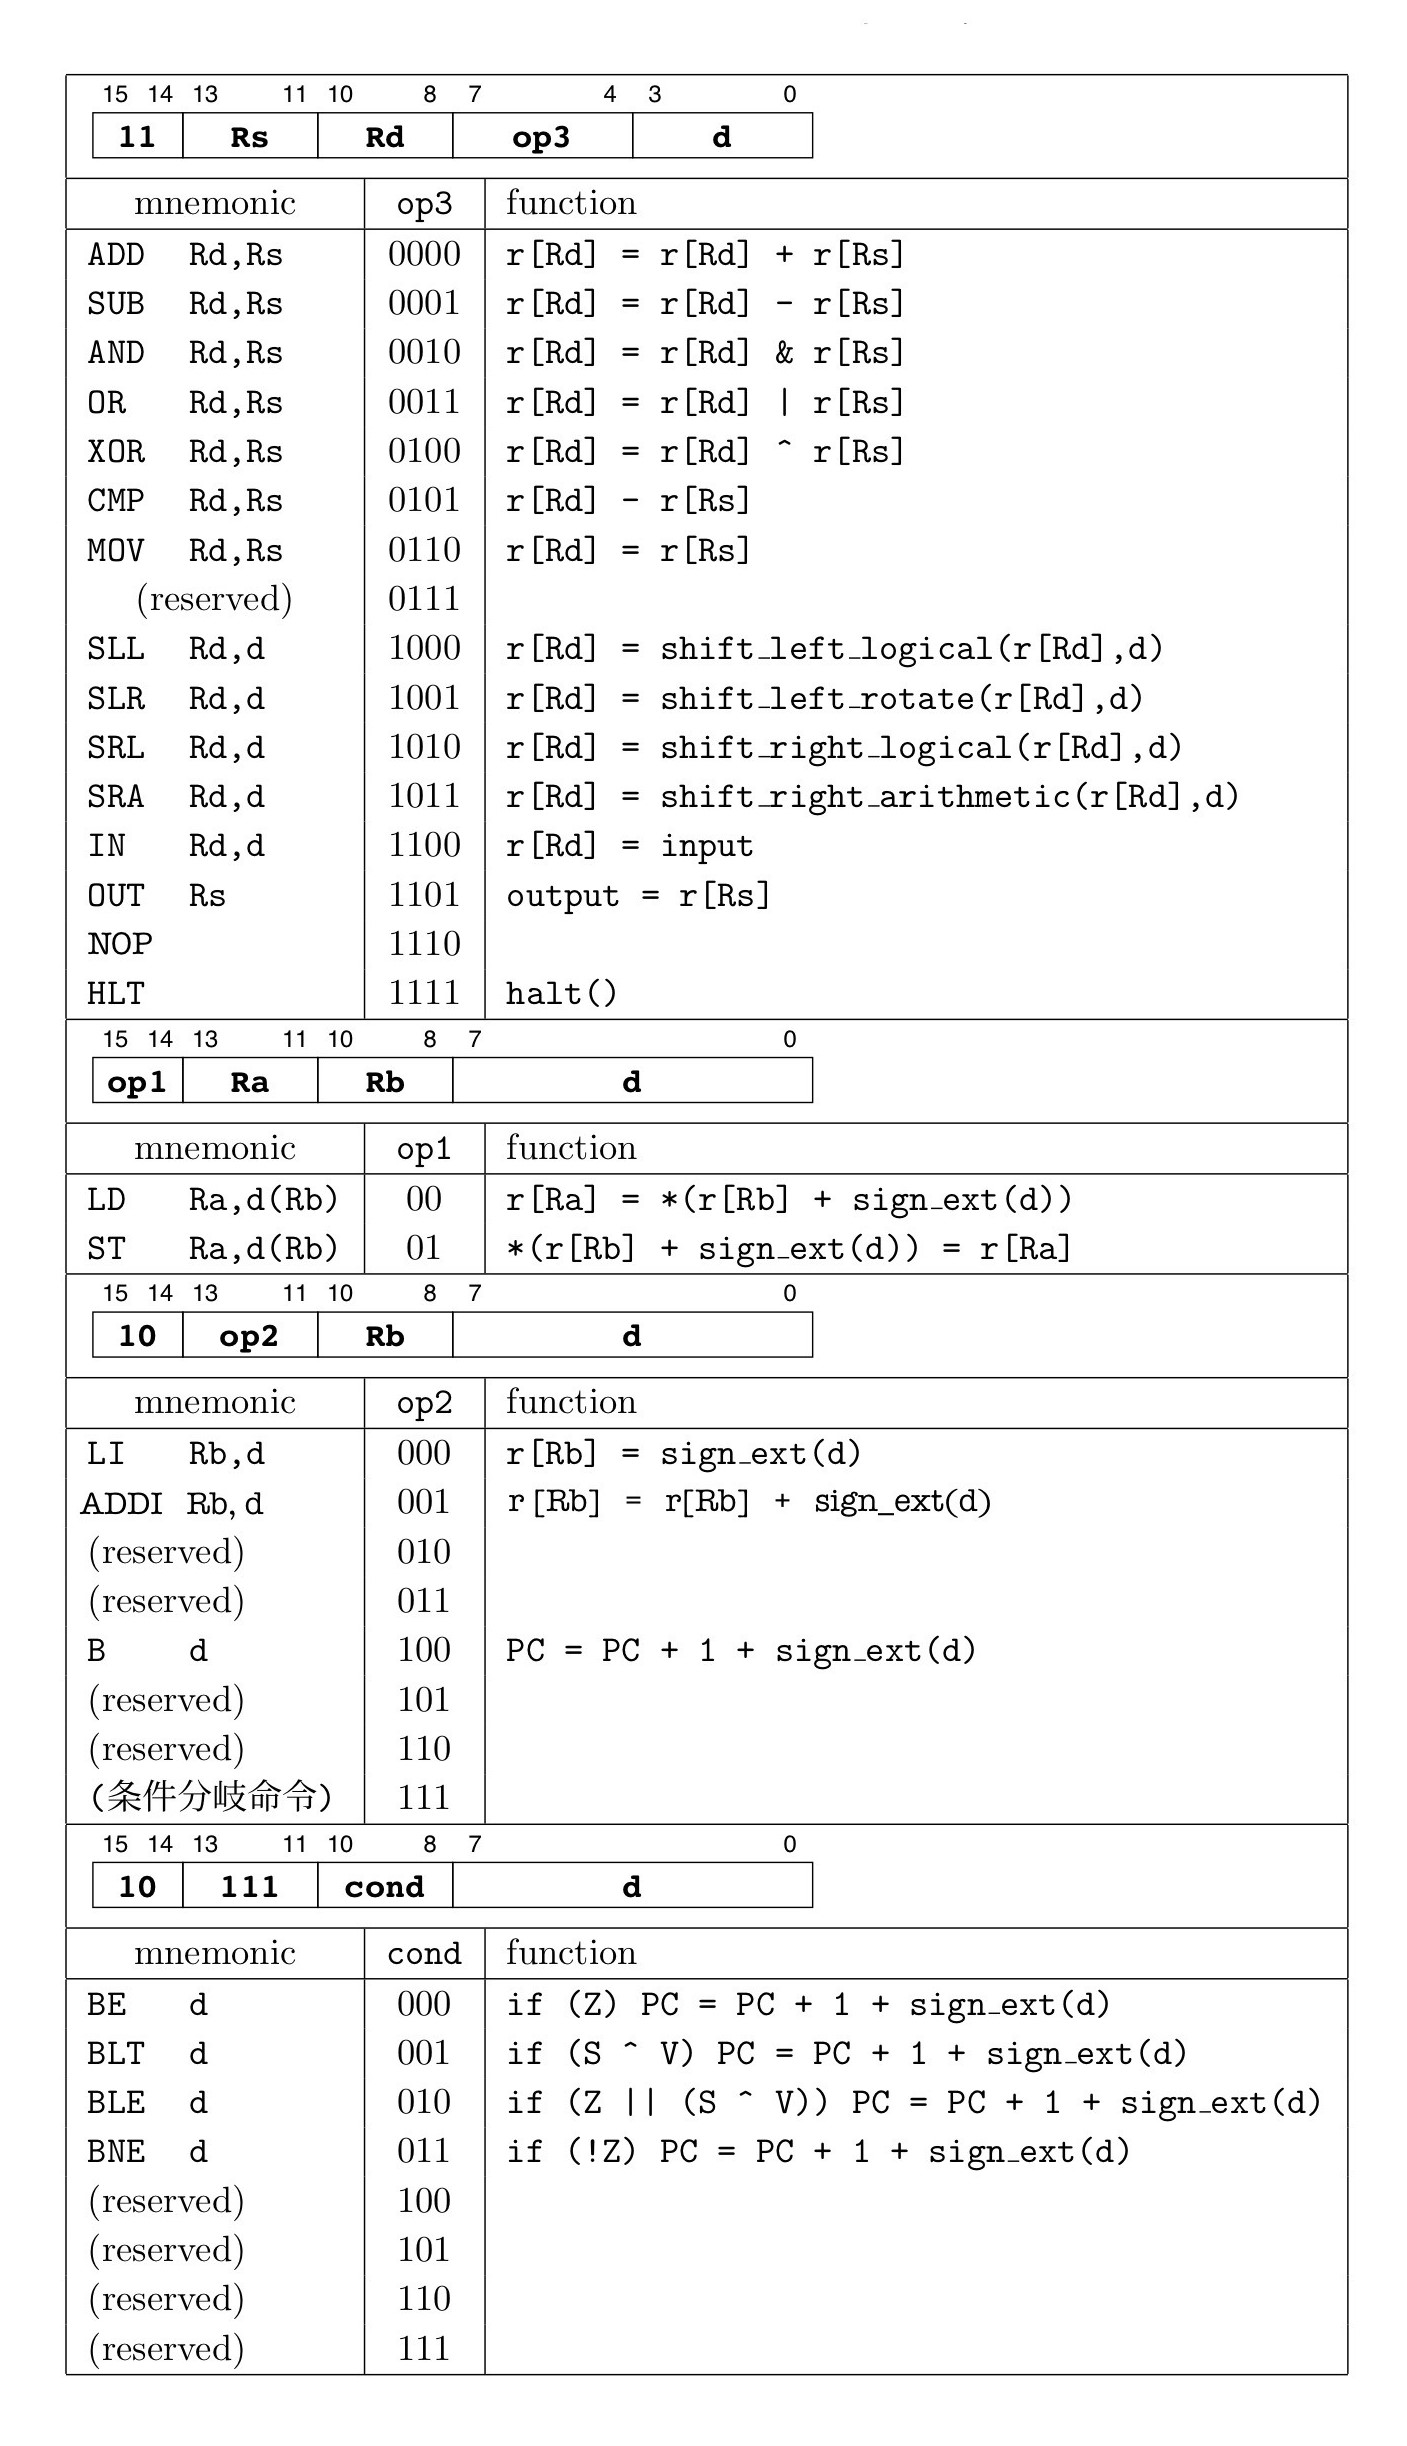
\includegraphics[scale = 0.22]{instructionSet.jpg}
    \end{center}
    \caption{命令セット・アーキテクチャ}
    \label{instructionSet}
\end{figure}

\subsection{IN命令}
IN命令が呼ばれると実行を一時的に中断し、外部入力で入力された値をうけとる。
中間発表の段階の外部入力では、実行の中断中に16個のディップスイッチを変更し、16bitの値を設定し、
execボタンを押すことでexecボタンが押された時のディップスイッチを用いて表現された値を入力として受け取り、
実行を再開するようにした。

\subsection{OUT命令}
OUT命令が呼ばれると、フェーズがp3の時に外部出力にRsフィールドで指定したレジスタの中身が渡される。
中間発表の段階の外部出力では7SEG-LEDを4つ用いて16進数表示で16bitのデータを表示する。
また、過去16回のOUT命令で出力されたデータを保持し、7SEG-LEDに表示する。

\subsection{HLT命令}
命令の実行を中断するための命令である。内部的にはexecボタンが押されたのと同じ動作をする。
HLT命令が呼ばれた後に、execボタンを押すとメモリ上でHLT命令の次の命令から命令の実行を再開する。

\subsection{NOP命令(=non operation)}
レジスタ・メモリ書き込み、外部入出力などの動作を、何も行わない命令である。機器の初期化の際に、
resetボタンが押されるとInstruction Registerの値は2'b 1100000011100000となり、NOP命令の値に設定される。

\subsection{ADDI命令}
Rbフィールドで指定したレジスタの中身を読み出し、命令の下8bitで指定した符号付きの値dを足し合わせる。
足し合わせた値をRbフィールドで指定したレジスタに格納する。
中間発表の段階では未実装の機能である。

\subsection{その他の命令}
ADD,SUB,AND,OR,XOR,CMP,MOV,SLL,SLR,SRL,SRA,LD,ST,LI,B,BE,BLT,BLE,BNEについては授業資料の命令セットの仕様通りに設計を行ったため、
授業資料の命令セットの説明と被る箇所は割愛する(授業資料のコピーを載せることになるので割愛)。
ただし、LD,ST,LI,IN,OUT命令でのSZCVのフラグについて、
それぞれの命令で移動するデータの値(LDならばメモリからロードするデータ、STならばメモリに格納するデータ、
LIならばレジスタに格納する即値の値、INならば入力として受け取るデータ、OUTならば出力するデータ)が、
正のときSZCV=0000、負のときSZCV=1000、0のときSZCV=0100となるようにSZCVフラグを設定した。


\section{構造と動作}
現状のプロセッサの構造は以下の図\ref{structure0506}のようになる。

\begin{figure}[H]
    \begin{center}
    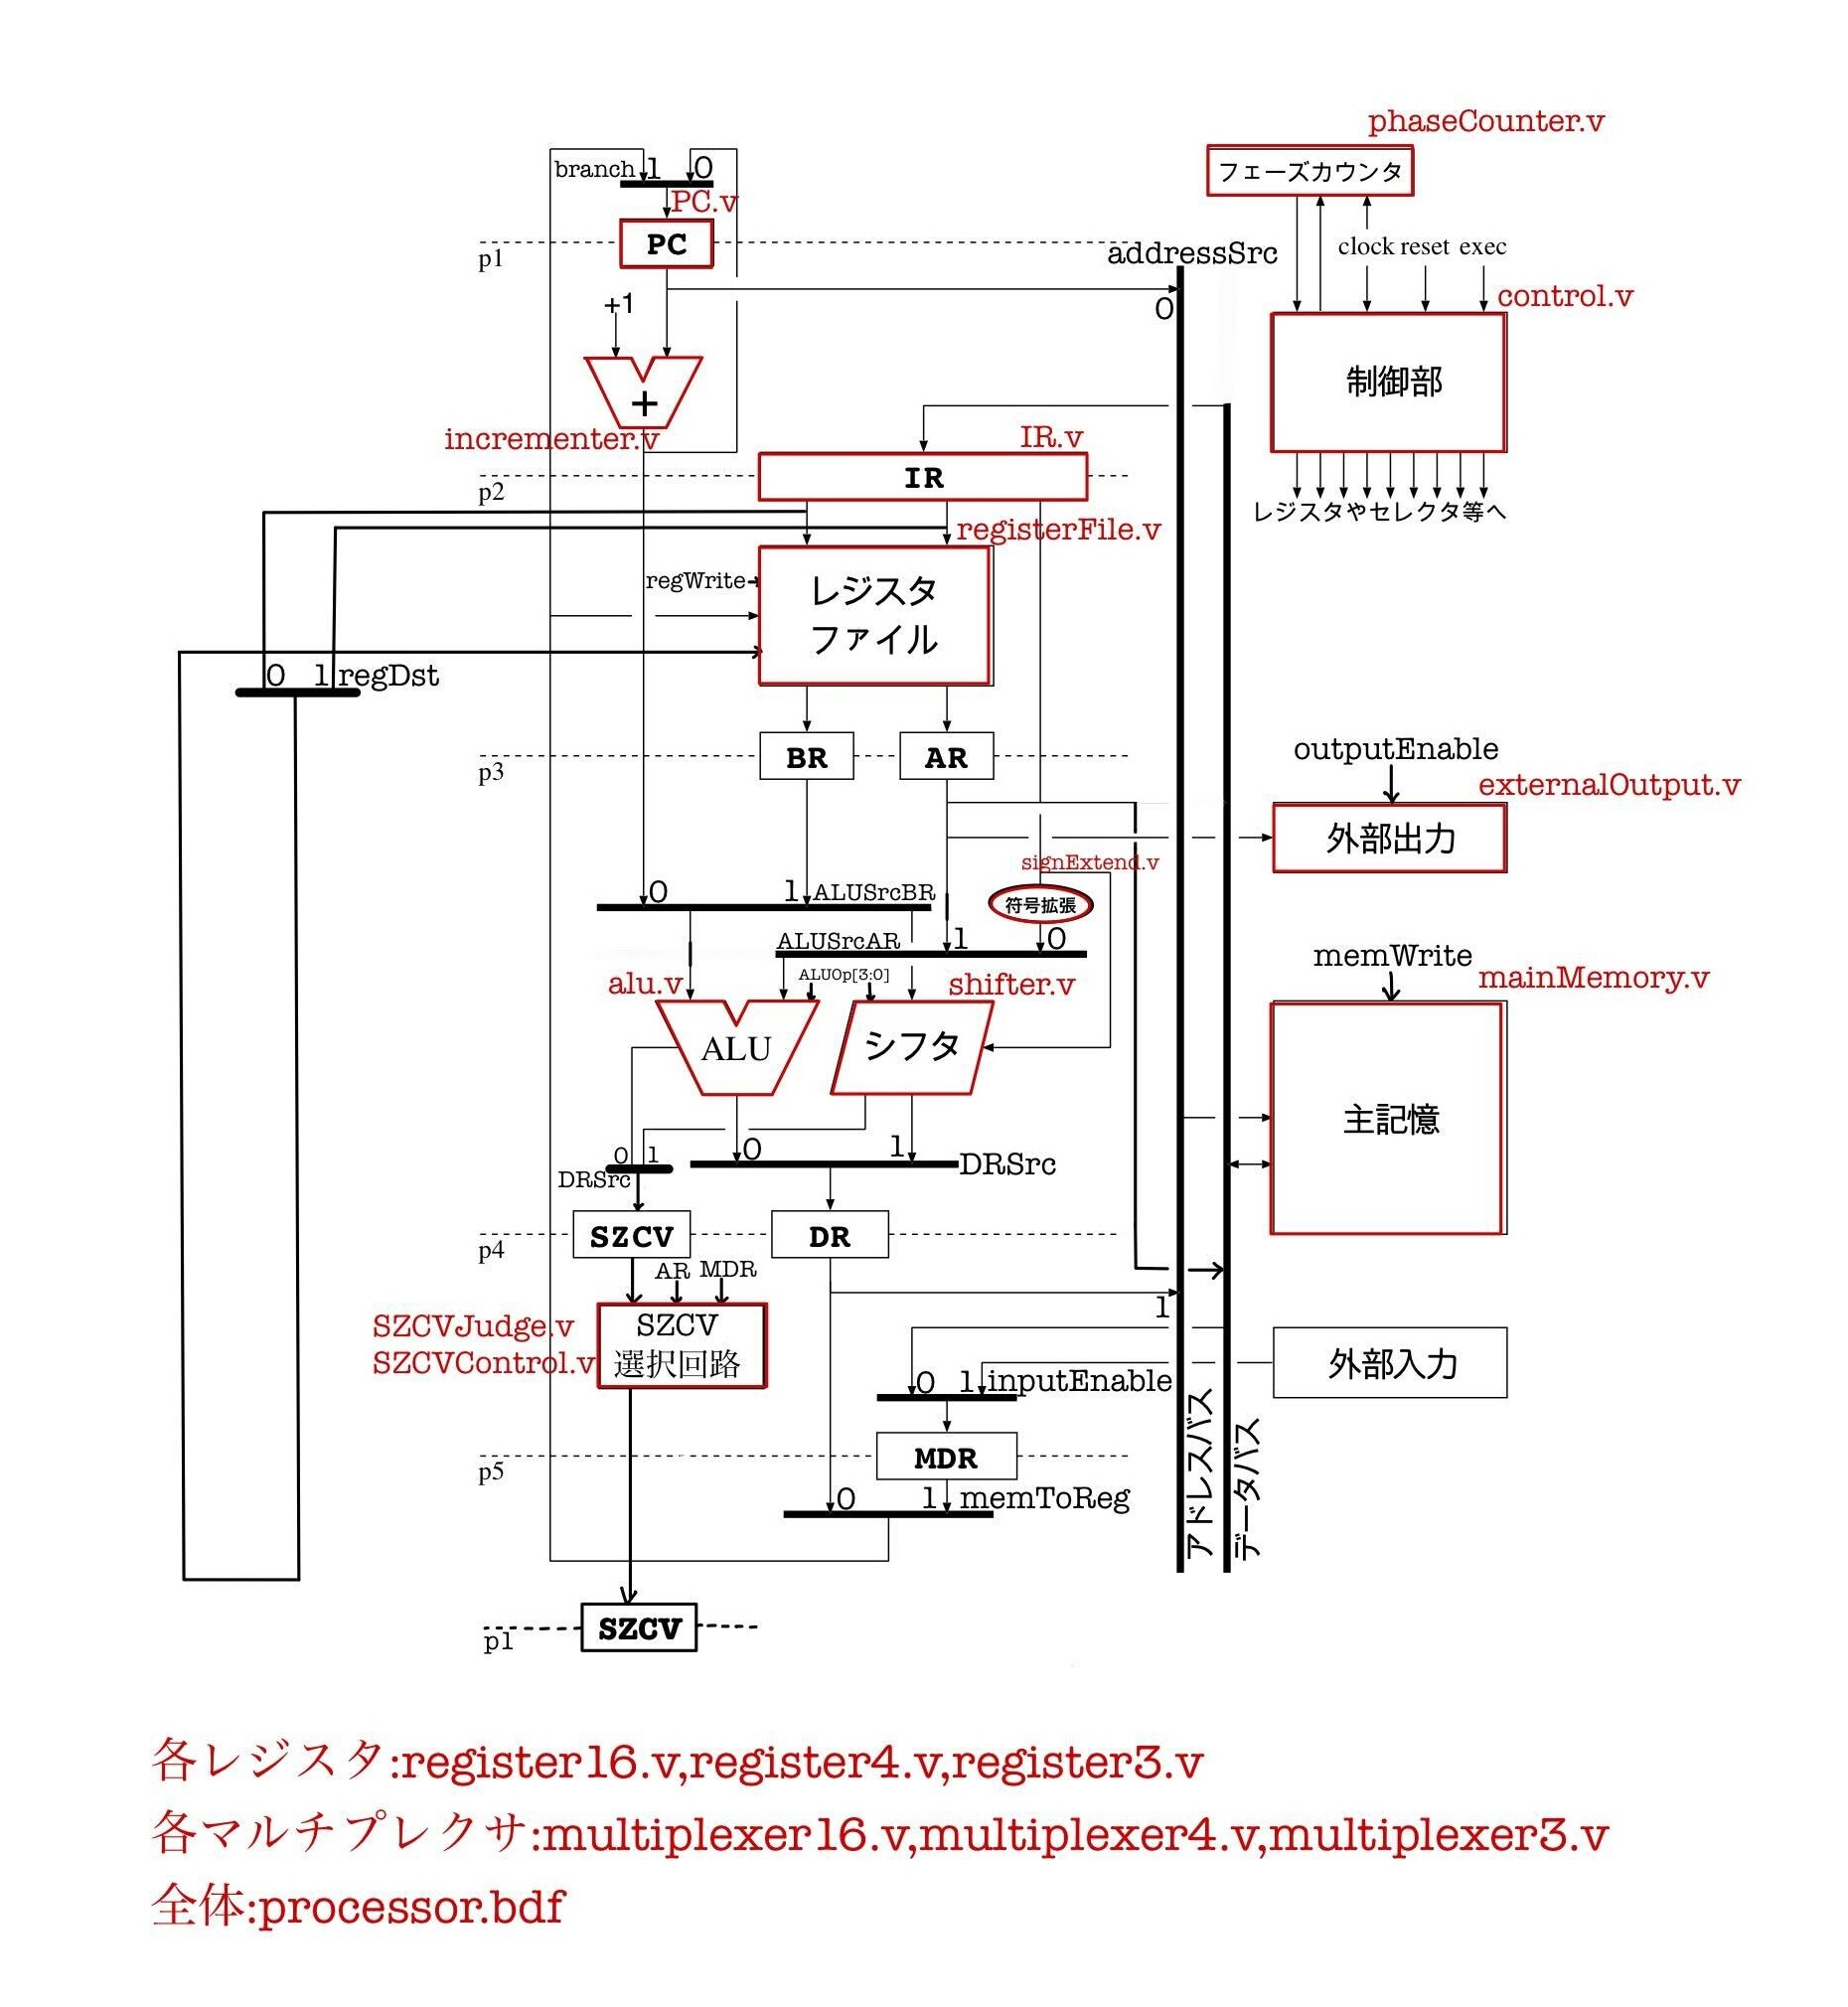
\includegraphics[scale = 0.22]{structure0506.jpg}
    \end{center}
    \caption{プロセッサの構造(現状)}
    \label{structure0506}
\end{figure}



このプロセッサは5フェーズに処理をわけ、
フェーズカウンタによりクロックサイクルごとに
p1,p2,p3,p4,p5というフェーズ信号が順に立ち上がる。
それぞれのフェーズ信号は図\ref{structure0506}の破線上の
レジスタのイネーブル信号として入力される。
レジスタのイネーブル信号とは、クロックの立ち上がりでかつ、
レジスタのイネーブル信号が1であるときのみ、レジスタの中身が書き変わるような信号である。
これにより、各フェーズの書き換えをしたいレジスタのみが順に書き変わっていき、処理が実現する。

このプロセッサは制御部内にSystemRunningという1bitのレジスタをもっており、
そのレジスタの値が0のときにSystemRunningレジスタ以外のすべてのレジスタのイネーブル信号が0になるようになっている。
execボタンを押されると、このSystemRunningの反転が行われる。
これによりexecボタンを押すたびに実行停止・再開ができる。
resetボタンを押すと、以下のことがすべて行われる。
\begin{itemize}
\item IRにNOP命令を表す命令コード2'b 1100000011100000が格納される。
\item PCに0が格納される。
\item 外部出力の過去の出力履歴がクリアされる。
\item レジスタファイルの内部のレジスタに0が格納される。
\item フェーズカウンタのフェーズ信号をp1に戻す。
\item SystemRunningに0が格納される。
\end{itemize}
これによりresetボタンを押すことで機器を初期状態にし、実行待機状態にすることができる。
この状態でexecボタンを押すとメモリの0番地から順に命令が実行される。
FPGAにプログラムをダウンロードした後にexecボタンを押さなければ、
命令が実行されないことに注意が必要である。

以下はまだ実現されていない機能であるが、
このプロセッサにパイプライン処理を追加する。
p1からp5の5フェーズを並列に実行する。
パイプライン化により、プロセッサの動作は変えずに、処理の高速化を行う。
構造については、以下の変更をする。
\begin{itemize}
\item メモリを命令メモリとデータメモリに分け、構造ハザードを防ぐ。
\item ALUとは別にアドレス計算用の加算器を用意し、アドレス計算と演算の際のALUでの構造ハザードを防ぐ。
\item 各フェーズの間にレジスタを用意し、フェーズ間での制御信号やデータの受け渡しを行う。
\item データのフォーワーディングをおこなうフォーワーディングユニットを追加する。
\item パイプラインストールを防止するハザード検出ユニットを追加する。
\item 分岐ハザードに対処する回路を追加する。
\item 必要な制御信号の追加や、制御信号の変更を行う。
\item フェーズカウンタを削除する。
\end{itemize}
これらの変更を行い実装をする。
パイプライン化の構造の具体的な設計はまだできていないので、
最終課題で報告する。

\end{document}
